
\noindent \textcolor{COLOR1}{Questão 03)} Numa empresa existem três máquinas para produzir um certo tipo de peça. Foram retiradas amostras aleatórias de dimensão cinco de cada uma das máquinas e foi medido o diâmetro (em mm) de cada uma das peças, resultando nos resultados abaixo:

\begin{itemize}
    \item Máquina 1: $49, 55, 51, 52, 48$;
    \item Máquina 2: $53, 54, 58, 49, 56$;
    \item Máquina 3: $55, 51, 52, 52, 52, 50$;
\end{itemize}

Verifique se existem diferenças entre os diâmetros das peças produzidas por cada uma das máquinas. No caso de haver diferenças, quais os pares de máquinas responsáveis por essas diferenças?
\\

Para o caso em questão, tomemos como hipóteses:
\begin{itemize}
    \item $H_0:$ Máquina 1, 2 e 3 têm média de diâmetro iguais;
    \item $H_a:$ Pelo menos uma das máquinas possui a média de diâmetro diferente;
\end{itemize}

Temos o seguinte boxplot para esses dados:\\

\begin{figure}[htbp]
    \centering
    \subfloat{{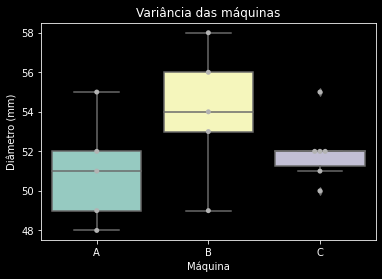
\includegraphics[scale=.8]{/estatistica/anova-boxplot.png} }}%
\end{figure}

\begin{lstlisting}
import pandas as pd
import statsmodels.api as sm
from statsmodels.formula.api import ols
import matplotlib.pyplot as plt
import seaborn as sns
plt.style.use('dark_background')

# dados
data = {"A": {0: 49, 1: 55, 2: 51, 3: 52, 4: 48}, 
        "B": {0: 53, 1: 54, 2: 58, 3: 49, 4: 56}, 
        "C": {0: 55, 1: 51, 2: 52, 3: 52, 4: 52, 5: 50}
        }
df = pd.DataFrame(data)

df_melt = pd.melt(df.reset_index(), id_vars=["index"],
value_vars=["A", "B", "C"])

df_melt.columns = ["index", "treatments", "value"]

ax = sns.boxplot(data=df)
ax = sns.swarmplot(data=df, color=".7")
ax.title.set_text("Variancia das maquinas")
ax.set_xlabel("Maquina")
ax.set_ylabel("Diametro (mm)")

plt.figure()

#Obter tabela com valores da anova
model = ols("value ~ treatments", data=df_melt).fit()
anova_table = sm.stats.anova_lm(model, typ=2)
anova_table
\end{lstlisting}

Obtém-se a seguinte tabela com os valores da análise de variância:
\\

\begin{table}[ht]
    \centering
    \begin{tabular}{c|c|c|c|c}
        \hline
        \rowcolor{pagecolor!50!COLOR1}
                   & sum\_sq & df   & F        & PR(\textgreater{}F) \\ \hline
        treatments & 23.4375 & 2.0  & 1.692708 & 0.222156            \\ \hline
        residual   & 90.0    & 13.0 & NaN      & NaN                 \\ \hline
    \end{tabular}
\end{table}

A partir da tabela com dados gerados, pode-se concluir então que o valor de $p$ (ou $PR(>F)$) obtido a partir da análise ANOVA é, significantemente maior que $0.05$. Não se rejeita a hipótese $H_0$ de que as médias dos três grupos de dados são iguais.